
\setcounter{section}{0}
\setcounter{viduii}{0}
	\viduii{3}{
	Một chiếc hộp gỗ được thả trượt không vận tốc ban đầu, từ đầu trên của một tấm gỗ dài $L=\SI{2}{m}$. Tấm gỗ đặt nghiêng $30^\circ$ so với phương ngang. Hệ số ma sát giữa đáy hộp và mặt gỗ là $\SI{0.2}{}$. Lấy $g=\SI{9.8}{m/s^2}$. Hỏi sau bao lâu thì hộp trượt xuống đến đầu dưới của tấm gỗ?
}
{	\begin{center}
		\textbf{Hướng dẫn giải}
	\end{center}
	\begin{center}
		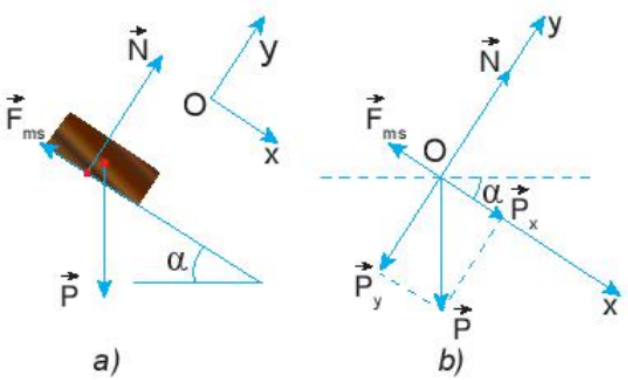
\includegraphics[scale=0.5]{../figs/G10-17-3}
	\end{center}
	
	\begin{itemize}
		\item Hộp gỗ (coi là chất điểm) chịu tác dụng của ba lực: trọng lực $\vec P$, phản lực $\vec N$ và lực ma sát $\vec F_\text{ms}$.
		
		\item Chọn hệ trục tọa độ: O$x$, O$y$ như hình vẽ. Phân tích trọng lực $\vec P$ thành hai lực thành phần $\vec P_x$, $\vec P_y$.
		
		Phương trình định luật II Niu-tơn:
		\begin{equation}\label{10}
			\vec F_\text{ms} + \vec P_x + \vec P_y + \vec N = m \vec a
		\end{equation}
		
		\item Chiếu các vectơ lực lên các trục tọa độ đã chọn:
		
		Chiếu ($\ref{10}$) lên O$x$:
		\begin{equation}\label{11}
			mg \sin \alpha - F_\text{ms} = ma \\
		\end{equation}
		
		Chiếu (\ref{10}) lên O$y$:
		\begin{equation}\label{12}
			N - mg \cos \alpha = 0
		\end{equation}
		\begin{equation}\label{13}
			F_\text{ms} = \mu N
		\end{equation}
		Giải hệ phương trình trên, ta có:
		\begin{equation*}
			a = g(\sin \alpha - \mu \cos \alpha)
		\end{equation*}
		
		Thay số, ta được $a \approx \SI{3.2}{m/s}$. Vậy hộp trượt xuống với gia tốc $a=\SI{3.2}{m/s^2}$, cùng chiều với trục O$x$.
		
		\item Áp dụng công thức xác định thời gian trong chuyển động thẳng biến đổi đều:
		$$t=\sqrt{\dfrac{2L}{a}} \approx \SI{1.1}{s}$$
	\end{itemize}
}
	\viduii{4}{Hay vật 1 và 2 có thể trượt trên mặt bàn nằm ngang và được nối với nhau bằng dây không dãn, khối lượng dây không đáng kể. Khối lượng của các vật là $m_1 = \SI{2}{kg}$, $m_2=\SI{1}{kg}$. Tác dụng vào vật 1 lực $F=\SI{9}{N}$ theo phương song song với mặt bàn. Hệ số ma sát giữa hai vật với mặt bàn là $\mu=\SI{0.2}{}$. Lấy $g=\SI{10}{m/s^2}$. Hãy tính gia tốc chuyển động của các vật.
}
{	\begin{center}
		\textbf{Hướng dẫn giải}
	\end{center}
	\begin{center}
		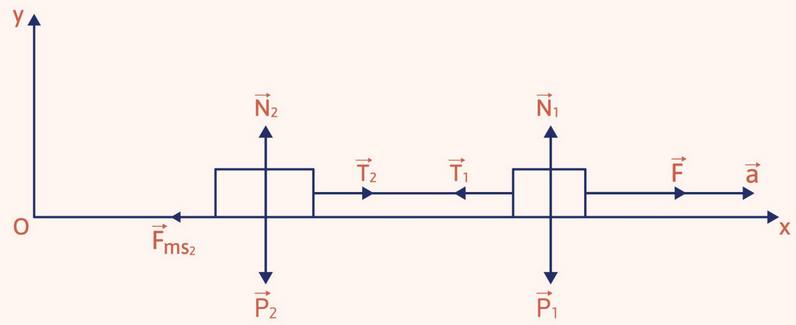
\includegraphics[scale=0.5]{../figs/G10-17-2}
	\end{center}
	
	\begin{itemize}
		\item Đối với vật 1:
		\begin{equation}\label{1}
			\vec P_1 + \vec N_1 + \vec T_1 + \vec F_\text{ms1} + \vec F = m_1 \vec a_1
		\end{equation}
		
		Chiếu (\ref{1}) xuống O$x$: $F - T_1 - F_\text{ms1} = m_1 a_1$.
		
		Chiếu (\ref{1}) xuống O$y$: $-m_1 g + N_1 = 0$.
		
		Với $F_\text{ms1} = \mu N_1 = \mu m_1 g$, suy ra:
		\begin{equation}\label{2}
			F-T_1 - \mu m_1 g = m_1 a_1
		\end{equation}
		\item Đối với vật 2:
		\begin{equation}\label{3}
			\vec P_2 + \vec N_2 + \vec T_2 + \vec F_\text{ms2} + \vec F = m_2 \vec a_2
		\end{equation}
		
		Chiếu (\ref{3}) xuống O$x$: $T_2 - F_\text{ms2} = m_2 a_2$.
		
		Chiếu (\ref{3}) xuống O$y$: $-m_2 g + N_2 = 0$.
		
		Với $F_\text{ms2} = \mu N_2 = \mu m_2 g$, suy ra:
		\begin{equation}\label{4}
			T_2 - \mu m_2 g = m_2 a_2
		\end{equation}
		
		\item Do khối lượng dây không đáng kể nên $T_1 = T_2 = T$, do dây không dãn nên $a_1 = a_2 = a$.
		
		Biến đổi (\ref{2}), ta được:
		\begin{equation}\label{5}
			F - T - \mu m_1 g = m_1 a
		\end{equation}
		
		Biến đổi (\ref{4}), ta được:
		\begin{equation}\label{6}
			T - \mu m_2 g= m_2 a
		\end{equation}
		
		\item Cộng (\ref{5}) và (\ref{6}), ta được:
		\begin{equation*}
			F - \mu (m_1 + m_2) g = (m_1 + m_2) a \\
			\Rightarrow a = \dfrac{F - \mu (m_1 + m_2)g}{m_1 + m_2} = \SI{1}{m/s^2}
		\end{equation*}
	\end{itemize}
}
\begin{enumerate}[label=\bfseries Câu \arabic*:]
		\item \mkstar{2}
	
	{
		Một ô tô có khối lượng 2 tấn bắt đầu chuyển động. Sau khi đi được 20 giây thì ô tô đạt tốc độ $\SI{72}{km/h}$. Biết hệ số ma sát giữa bánh xe và mặt đường là $\SI{0.2}{}$, lấy $g=\SI{10}{m/s^2}$. Tính lực phát động của ô tô.
	}
	
	\hideall{
		
		Gia tốc của ô tô thu được:
		$$a=\dfrac{\Delta v}{\Delta t} = \SI{1}{m/s^2}$$
		
		Áp dụng định luật II Niu-tơn:
		$$F-F_\text{ms} = ma \Rightarrow F - \mu m g = ma \Rightarrow F = \SI{6000}{N}$$
	}
	
	\item \mkstar{2}
	
	{
		Tác dụng một lực có độ lớn $\SI{10}{N}$ vào một vật nặng $\SI{2}{kg}$ đang đứng yên, làm cho vật chuyển động thẳng nhanh dần đều. Bỏ qua ma sát, hãy tính gia tốc của vật và quãng đường mà vật đi được trong 20 giây.
	}
	
	\hideall{
		
		Gia tốc mà vật thu được:
		$$a=\dfrac{F}{m} = \SI{5}{m/s^2}$$
		
		Quãng đường mà vật đi được trong $\SI{20}{s}$:
		$$s=\dfrac{1}{2}at^2 = \SI{1000}{m}.$$
	}
	\item \mkstar{2}
	
	
	{
		Vật khối lượng m đặt trên mặt phẳng nghiêng hợp với phương nằm ngang một góc $\alpha$. Hệ số ma sát trượt giữa vật và mặt phẳng nghiêng là $\mu_\text{t}$. Khi được thả ra, vật trượt xuống. Gia tốc của vật phụ thuộc vào những đại lượng nào?
		
	}
	
	\hideall
	{
			\begin{center}
				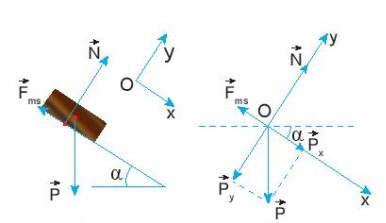
\includegraphics[scale=1]{../figs/VN10-2022-PH-TP021-3.jpg}
			\end{center}
		Theo định luật 2 Newton:
		
		$$ \vec F_\text{ms} + \vec P + \vec N = m\vec a.$$
		
		
		
		Áp dụng định luật 2 Newton theo hai trục Ox, Oy:
		
		$$\begin{cases}
			\text{Ox}:  mg\sin \alpha - \mu N= ma\ (1).\\
			\text{Oy}: 	N - mg\cos \alpha = 0\ (2).
		\end{cases}$$
		
		Thay (2) và (1) suy ra:
		
		$$a = g(\sin \alpha - \mu_\text{t} \cos \alpha).$$
	}
	\item \mkstar{2}
	
	
	{
		\begin{center}
			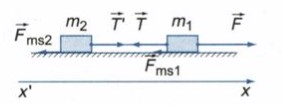
\includegraphics[scale=1]{../figs/VN10-2022-PH-TP021-19.jpg}
		\end{center}
		Hãy viết công thức của định luật II Newton cho mỗi vật.
		
	
	}
	
	\hideall
	{
	$$\begin{cases}
		\text{Vật 1:} m_1a = F - T - F_\text{ms1}.\\
		\text{Vật 2:} m_2a = T' - F_\text{ms2}.
	\end{cases}$$
	}
		\item \mkstar{2}
	
	
	{Cho hệ vật như hình. Biết $m_\text{A} > m_\text{B}$. Gia tốc của hai vật là $a$. Lực căng dây bằng bao nhiêu?
		\begin{center}
			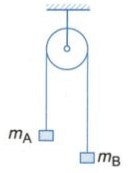
\includegraphics[scale=1]{../figs/VN10-2022-PH-TP021-22.jpg}
		\end{center}
	}
	
	\hideall{
		\begin{center}
			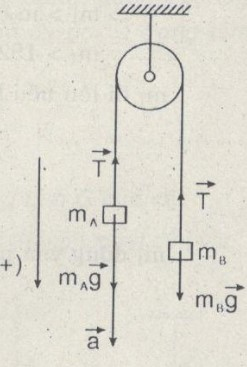
\includegraphics[scale=1]{../figs/VN10-2022-PH-TP021-23.jpg}
		\end{center}
		Áp dụng định luật II Newton cho vật $m_\text{A}$:
		
		$$m_\text{A} \vec a = m_\text{A} \vec g + \vec T$$
		
		Chiếu lên chiều dương ta được:
		
		$$ m_\text{A} a = m_\text{A} g - T \Rightarrow T = m_\text{A} (g-a).$$
	}
	\item \mkstar{3}
	
	{
		Một người đẩy một thùng hàng, khối lượng $\SI{50}{kg}$, trượt trên sàn nhà. Lực đẩy có phương nằm ngang với độ lớn là $\SI{180}{N}$. Tính gia tốc của thùng hàng, biết hệ số ma sát trượt giữa thùng hàng và sàn nhà là 0,25. Lấy $g = \SI{9,8}{m/s}^2$.
	}
	
	\hideall{
		\begin{center}
			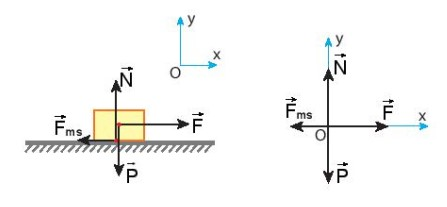
\includegraphics[scale=1]{../figs/VN10-2022-PH-TP021-1.jpg}
		\end{center}
		Thùng hàng chịu tác dụng của bốn lực: trọng lực $\vec P$, lực đẩy $\vec F$, phản ứng $\vec N$ và lực ma sát trượt $\vec F_\text{ms}$ của sàn.
		
		Coi thùng hàng như một chất điểm.
		
		Áp dụng định luật 2 Newton cho chuyển động của vật theo hai trục Ox, Oy:
		
		$$\begin{cases}
			\text{Ox}: F_\text{x} = F - F_\text{ms} = ma_\text{x} = ma\ (1).\\
			\text{Oy}: F_\text{y} = N - P = 0\ (2).
		\end{cases}$$
	
		$$F_\text{ms} = \mu N.$$
		
		Giải hệ phương trình:
		
		$$N = mg = \SI{490}{N}.$$
		
		$$F_\text{ms} = \mu N = \SI{122,5}{N}.$$
		
		Gia tốc của vật:
		
		$$a = \dfrac{F - F_\text{ms}}{m} = \SI{1,15}{m/s}^2.$$
		
		Thùng hàng trượt với gia tốc $a = \SI{1,15}{m/s}^2$ cùng chiều với trục Ox.
	
		
	
	}
	
	\item \mkstar{3}
	
	
	{Một người dùng dây buộc để kéo một thùng gỗ theo phương nằm ngang bằng một lực $\vec F$. Khối lượng của thùng $\SI{35}{kg}$. Hệ số ma sát giữa sàn và đáy thùng là 0,3. Lấy $g=\SI{9,8}{m/s}^2$.
		\begin{center}
			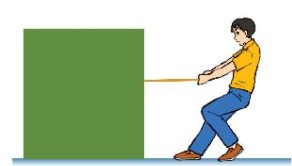
\includegraphics[scale=1]{../figs/VN10-2022-PH-TP021-2.jpg}
		\end{center}
	
	Tính độ lớn của lực kéo trong hai trường hợp:
	\begin{enumerate}[label=\alph*)]
		\item  Thùng trượt với gia tốc $\SI{0,2}{m/s}^2$.
		\item Thùng trượt đều.
	\end{enumerate}
	}
	
	\hideall
	{
	\begin{center}
		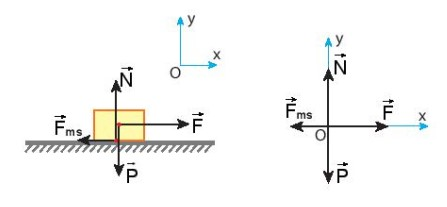
\includegraphics[scale=1]{../figs/VN10-2022-PH-TP021-1.jpg}
	\end{center}

	Coi thùng như một chất điểm và áp dụng định luật 2 Newton cho các lực thành phần theo các phương Ox, Oy.
	
	$$\begin{cases}
		\text{Ox}: F_\text{X} = F - F_\text{ms} = ma_\text{x} = ma\ (1).\\
		\text{Oy}: F_\text{y} = N - P =0\ (2).
	\end{cases}$$

	$$F_\text{ms} = \mu N.$$
	
	Giải hệ phương trình:
	
	Từ (2) suy ra $N = mg$.
	
	Lực ma sát có giá trị:
	
	$$F_\text{ms} = \mu N = \mu mg.$$
	
	\begin{enumerate}[label=\alph*)]
		\item  Thùng trượt với gia tốc $\SI{0,2}{m/s}^2$
		
		$$F = m(a + \mu h) = \SI{109,9}{N}.$$
		\item Thùng trượt đều ($a =0$)
		
		$$F = \mu mg = \SI{102,9}{N}.$$
		
	\end{enumerate}

	
	}
	\item \mkstar{3}
	
	
	{
		Một chiếc hộp gỗ được thả trượt không vận tốc ban đầu, từ đầu trên của một tấm gỗ dài $L = \SI{2}{m}$. Tấm gỗ đặt nghiêng $30^\circ$ so với phương ngang. Hệ số ma sát giữa đáy hộp và mặt gỗ là 0,2. Lấy $g = \SI{9,8}{m/s}^2$. Hỏi sau bao lâu thì hộp trượt xuống đến đầu dưới của tấm gỗ?
	}
	
	\hideall
	{
		\begin{center}
			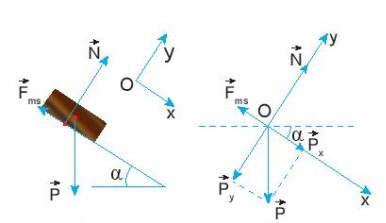
\includegraphics[scale=1]{../figs/VN10-2022-PH-TP021-3.jpg}
		\end{center}
		
		Áp dụng định luật 2 Newton theo hai trục Ox, Oy:
		
		$$\begin{cases}
			\text{Ox}: F_\text{x} = mg\sin \alpha - F_\text{ms}= ma_\text{x} = ma\ (1).\\
			\text{Oy}: F_\text{y} = N - mg\cos \alpha = 0\ (2).
		\end{cases}$$
	
		$$F_\text{ms} = \mu N.$$
		
		Giải hệ phương trình:
		
		$$a = g(\sin \alpha - \mu \cos \alpha).$$
		
		Thay số, ta được: $a \approx \SI{3,2}{m/s}^2$.
		
		Hộp trượt xuống với gia tốc $a = \SI{0,64}{m/s}^2$, cùng chiều với Ox. 
		
		Áp dụng công thức: 
		
		$$L  = \dfrac{1}{2}at^2 \Rightarrow t \approx \SI{1,1}{s}.$$
	}
	\item \mkstar{3}
	
	
	{
		Người ta đẩy một cái thùng có khối lượng $\SI{55}{kg}$ theo phương ngang với lực $\SI{220}{N}$ làm thùng chuyển động trên mặt phẳng ngang. Hệ số ma sát trượt giữa thùng và mặt phẳng là 0,35. Tính gia tốc của thùng. Lấy $g = \SI{9,8}{m/s}^2.$
	}
	
	\hideall
	{
		\begin{center}
			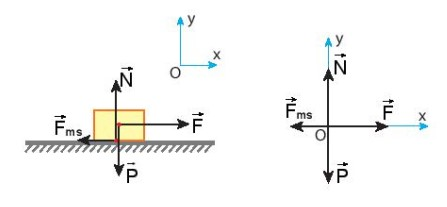
\includegraphics[scale=1]{../figs/VN10-2022-PH-TP021-1.jpg}
		\end{center}
	
		Chọn hệ quy chiếu và các lực có chiều như hình vẽ.
		
		Theo định luật 2 Newton:
		
		$$\vec F + \vec F_\text{ms} + \vec P + \vec N = m\vec a.$$
		
		Chiếu lên hệ trục tọa độ:
		
		$$\begin{cases}
			\text{Ox:} F - F_\text{ms} = ma \Leftrightarrow F - \mu N = ma.\ (*) \\
			\text{Ox:} P - N = 0 \Rightarrow N = P = mg.
			
		\end{cases}$$
	
		Thay $N = mg$ vào (*), ta có:
		
		$$F - \mu mg = ma \Rightarrow a = \dfrac{F - \mu mg}{m} = \SI{0,57}{m/s}^2.$$
		
	
	}
	\item \mkstar{3}
	
	
	{
		Một quyển sách đặt trên mặt bàn nghiêng và được thả cho trượt xuống. Cho biết góc nghiêng $\alpha = 30^\circ$ so với phương ngang và hệ số ma sát giữa quyển sách và mặt bàn là $\mu = \text{0,3}$. Lấy $g = \SI{9,8}{m/s}^2.$ Tính gia tốc của quyển sách và quãng đường đi được của nó sau $\SI{2}{s}$.
	}
	
	\hideall
	{
		\begin{center}
			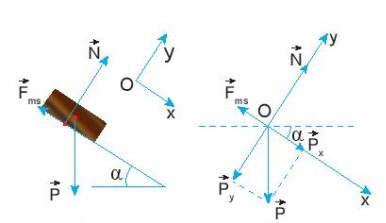
\includegraphics[scale=1]{../figs/VN10-2022-PH-TP021-3.jpg}
		\end{center}
		Theo định luật 2 Newton
		$$\vec F_\text{ms} + \vec P + \vec N = m\vec a.$$
		
		Chiếu lên hệ trục tọa độ:
		
		$$\begin{cases}
			\text{Ox:} P_\text{x} - F_\text{ms} = ma \Leftrightarrow mg\sin \alpha - \mu N = ma.\ (1) \\
			\text{Ox:}  N - P_\text{y}= 0 \Rightarrow N =mg \cos \alpha\ (2).
			
		\end{cases}$$
	
		Thay (2) vào (1) ta có:
		
		$$mg \sin \alpha - \mu mg \cos \alpha = ma \Rightarrow a = g \sin \alpha - \mu g \cos \alpha \approx \SI{2,35}{m/s}^2.$$
		
		Quãng đường nó đi được 
		
		$$S = \dfrac{1}{2}at^2 =\SI{4,7}{m}.$$
	}
	\item \mkstar{3}
	
	
	{
		Một học sinh dùng dây kéo một thùng sách nặng $\SI{10}{kg}$ chuyển động trên mặt sàn nằm ngang. Dây nghiêng một góc chếch lên trên $45^\circ$ so với phương ngang. Hệ số ma sát trượt giữa đáy thùng và mặt sàn là $\mu = \text{0,2}$ (lấy $g = \SI{9,8}{m/s}^2$). Hãy xác định độ lớn của lực kéo để thùng sách chuyển động thẳng đều.
	}
	
	\hideall
	{
		
		\begin{center}
			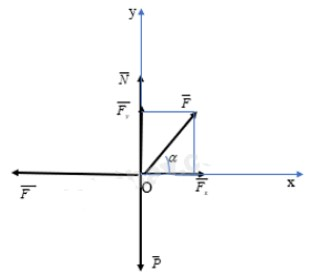
\includegraphics[scale=1]{../figs/VN10-2022-PH-TP021-12.jpg}
		\end{center}
	
			Theo định luật 2 Newton
		$$\vec F +\vec F_\text{ms} + \vec P + \vec N = m\vec a.$$
		
		Chiếu lên hệ trục tọa độ:
		
		$$\begin{cases}
			\text{Ox:} F_\text{x} - F_\text{ms} = ma \Leftrightarrow F\cos \alpha - \mu N = ma.\ (1) \\
			\text{Ox:}  N - P + F_\text{y}= 0 \Rightarrow N =P - F\sin \alpha\ (2).
			
		\end{cases}$$
	
		Mà $a = 0$ nên thay (2) vào (1) ta được:
		
		$$F\cos \alpha - \mu(P - F\sin \alpha) = 0 \Rightarrow F = \dfrac{\mu mg}{\cos \alpha + \mu \sin \alpha} \approx \SI{23,1}{N}.$$
		
		
	}
	\item \mkstar{3}
	
	
	{
		Hai vật có khối lượng lần lượt là $m_1 = \SI{5}{kg}$ và $m_2 = \SI{10}{kg}$ được nối với nhau bằng một sợi dây không dãn và được đặt trên một mặt sàn nằm ngang. Kéo vật 1 bằng một lực $\vec F$ nằm ngang có độ lớn $F = \SI{45}{N}$. Hệ số ma sát giữa mỗi vật và mặt sàn là $\mu = \text{0,2}$. Lấy $g = \SI{9,8}{m/s}^2$. Tính gia tốc của mỗi vật và lực căng của dây nối.
	}
	
	\hideall
	{
		\begin{center}
			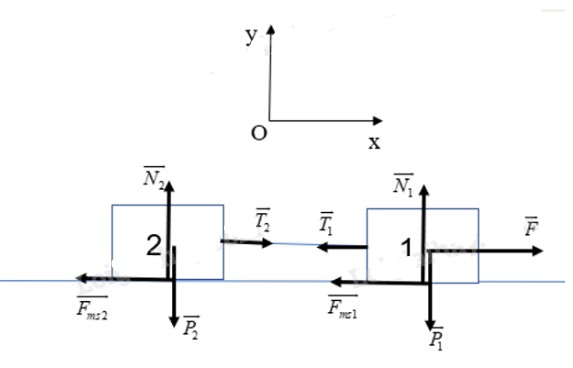
\includegraphics[scale=1]{../figs/VN10-2022-PH-TP021-13.jpg}
		\end{center}
	
	
		Chọn hệ quy chiếu như hình vẽ.
		
		Theo định luật 2 Newton cho hệ vật, ta có:
		
		$$\vec P_1 + \vec P_2 + \vec N_1 + \vec N_2 + \vec F + \vec F_\text{ms1} + \vec F_\text{ms2} + \vec T_1 + \vec T_2 = (m_1 + m_2)\vec a.\ (*)$$
		
		Chiếu (*) lên Ox, ta có
		
		$$F - F_\text{ms1} - F_\text{ms2} - T_1 + T_2 = (m_1 + m_2)a. \Rightarrow F - \mu(N_1 + N_2) = (m_1 + m_2)a\Rightarrow a = \dfrac{F - \mu (N_1 + N_2)}{m_1+m_2}\ (1).$$
		
		Chiếu (*) lên Oy, ta có
		
		$$N_1 + N_2 - P_1 - P_2 =0 \Rightarrow N_1 + N_2 = P_1 + P_2 \Rightarrow N_1 + N_2 = (m_1 + m_2)g\ (2).$$
		
		Thay (2) vào (1) ta được:
		
		 $$a = \dfrac{F - \mu (m_1 + m_2)g}{m_1+m_2}= \SI{1,04}{m/s}^2.$$
		
		Theo định luật 2 Newton, ta có
		
		$$\vec P_1 + \vec N_1 + \vec F + \vec F_\text{ms1} + \vec T_1 = m_1 \vec a\ (**).$$
		
		Chiếu (**) lên Ox, ta có:
		
		$$F - F_\text{ms1} - T_1 = m_1a.\ (3)$$
		Chiếu (**) lên Oy, ta có:
		
		$$N_1 = P_1 = m_1g. \ (4)$$
		
		Thay (4) vào (3) suy ra:
		
		$$T_1 = F - \mu m_1 g - m_1 a  = \SI{30}{N}.$$
		
		
	}
	\item \mkstar{3}
	
	
	{
		Một thùng hàng trọng lượng $\SI{500}{N}$ đang trượt xuống dốc. Mặt dốc tạo với phương ngang một gốc $30^\circ$. Chọn hệ tọa độ vuông góc xOy sao cho trục Ox theo hướng chuyển động của thùng.
		\begin{enumerate}[label=\alph*)]
			\item  Vẽ giản đồ vecto lực tác dụng lên thùng.
			\item Tính các thành phần của trọng lực theo các trục tọa độ vuông góc.
			\item Giải thích tại sao lực pháp tuyến của dốc lên thùng hàng không có tác dụng kéo thùng hàng xuống dốc.
			\item Xác định hệ số ma sát trượt giữa mặt dốc và thùng hàng nếu đo được gia tốc chuyển động của thùng là $\SI{2}{m/s}^2$. Bỏ qua lực cản của không khí lên thùng.
		\end{enumerate}
	}
	
	\hideall
	{
		
			\begin{enumerate}[label=\alph*)]
			\item  Vẽ giản đồ vecto lực tác dụng lên thùng.
			
			
			\begin{center}
				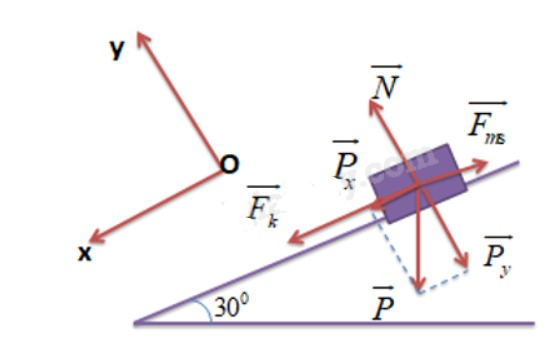
\includegraphics[scale=0.6]{../figs/VN10-2022-PH-TP021-14.jpg}
			\end{center}
			
			\item 
			Ta có:
			$$\begin{cases}
			P_\text{x}= P\sin \alpha = \SI{250}{N}.   \\
			P_\text{y}= P \cos \alpha = \xsi{250\sqrt 3}{N}.
			\end{cases}$$
			
			\item Lực pháp tuyến của dốc lên thùng hàng không có tác dụng kéo thùng hàng xuống dốc vì nó cân bằng với thành phần $\vec P_\text{y}$
			của trọng lực.
			
		
			\item Theo định luật 2 Newton
			$$\vec F_\text{ms} + \vec P + \vec N = m\vec a.$$
			
			Chiếu lên hệ trục tọa độ:
			
			$$\begin{cases}
				\text{Ox:}  P_\text{x} - F_\text{ms} =ma \Leftrightarrow  P_\text{x} - \mu N = ma.\ (1) \\
				\text{Oy:}  N - P_\text{y}= 0 \Rightarrow N =P_\text{y}\ (2).
				
			\end{cases}$$
		
			Thay (2) vào (1) ta được:
			
			$$ P_\text{x} - \mu P_\text{y} = ma \Rightarrow \mu = \dfrac{ P_\text{x}  -ma}{ P_\text{y}} \approx \SI{0,346}{0} $$
		\end{enumerate}
	}
	\item \mkstar{3}
	
	
	{
		Một học sinh đẩy một hộp đựng sách trượt trên sàn nhà. Lực đẩy ngang là $\SI{180}{N}$. Hộp có khối lượng $\SI{35}{kg}$. Hệ số ma sát trượt giữa hộp và sàn là 0,27. Hãy tìm gia tốc của hộp. Lấy $g = \SI{9,8}{m/s}^2$.
	}
	
	\hideall
	{
		\begin{center}
			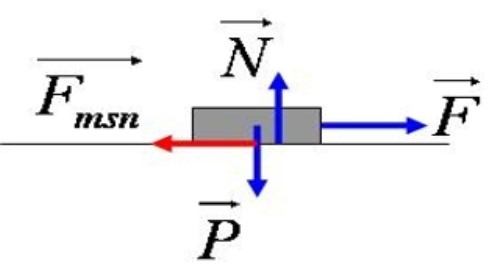
\includegraphics[scale=0.6]{../figs/VN10-2022-PH-TP021-4.jpg}
		\end{center}
	
	Áp dụng định luật II Newton theo hai trục toạ độ:
	
	$$\text{Ox}: F_\text{x} = F - F_\text{ms} = ma_\text{x} = ma.$$
	
	$$Oy: F_\text{y} = N - P = ma_\text{y} = 0.$$
	
	$$F_\text{ms} = \mu N.$$
	
	Giải hệ phương trình:
	
	$$N = P = mg = \SI{343}{N}.$$
	
	$$F_\text{ms} = \mu N = \SI{92,6}{N}.$$
	
	Gia tốc của vật
	
	$$a = \dfrac{F-F_\text{ms}}{m} = \SI{2,5}{m/s}^2.$$
	}
	\item \mkstar{3}
	
	
	{
		Một xe trượt không vận tốc đầu từ đỉnh mặt phẳng nghiêng góc $\alpha = 30^\circ$. Chiều dài mặt phẳng nghiêng là $l = \SI{1}{m}$. Lấy $g = \SI{10}{m/s}^2$ và hệ số ma sát 0,3464. Tính gia tốc chuyển động của vật.
		
		\begin{center}
			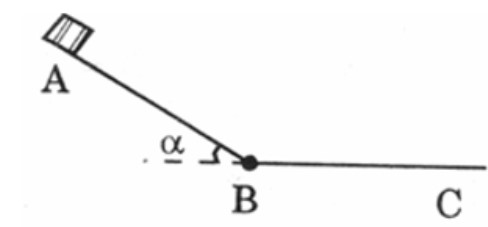
\includegraphics[scale=0.6]{../figs/VN10-2022-PH-TP021-5.jpg}
		\end{center}
	}
	
	\hideall
	{
		\begin{center}
			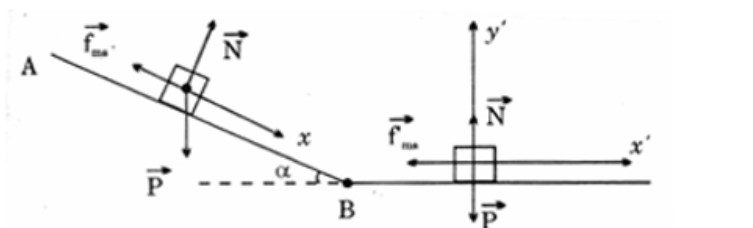
\includegraphics[scale=0.6]{../figs/VN10-2022-PH-TP021-6.jpg}
		\end{center}
	Các lực tác dụng vào vật:
	
	1. Trọng lực $\vec P$.
	
	2. Lực ma sát $\vec f_\text{ms}$.
	
	3. Phản lực $\vec N$ của mặt phẳng nghiêng.
	
	4. Hợp lực $\vec f_\text{ms} + \vec P + \vec N = m\vec a.$
	
	Chiếu lên trục Oy: 
	
	$$- P\cos \alpha + N = 0.$$
	
	$$\Rightarrow  N =mg \cos \alpha\ (1).$$
	
	Chiếu lên trục Ox: 
	
	$$P \sin \alpha - F_\text{ms} = ma_\text{x}.$$
	
	$$\Rightarrow  mg\sin \alpha  - \mu N = ma_\text{x}\  (2).$$
	
	Từ (1) và (2) 
	
	$$\Rightarrow mg\sin \alpha - mg \cos \alpha = ma_\text{x}.$$
	
	$$\Rightarrow a_\text{x} = g(\sin \alpha - \mu \cos \alpha) = \SI{2}{m/s}^2.$$
	}
	\item \mkstar{3}
	
	
	{
		Một quyển sách được thả trượt từ đỉnh của một bàn nghiêng một góc $\alpha = 35^\circ$ so với phương ngang. Hệ số ma sát trượt giữa mặt dưới của quyển sách với mặt bàn là $\mu = \text{0,5}$. Tìm gia tốc của quyển sách. Lấy $g = \SI{9,8}{m/s}^2$.
	}
	
	\hideall
	{
		Quyển sách chịu tác dụng của ba lực: trọng lực $\vec P$, lực pháp tuyến $\vec N$ và lực ma sát $\vec F_\text{ms}$ của mặt bàn.
		
		Áp dụng định luật II Niu-tơn theo hai trục toạ độ.
		
		$$\text{Ox}: F_\text{x} = P \sin \alpha - F_\text{ms} = ma_\text{x} = ma.$$
		
		$$\text{Oy}: F_\text{y} = N - P \cos \alpha = ma_\text{y} = .0$$
		
		$$F_\text{ms} = \mu N.$$
		
		Giải hệ phương trình ta được:
		
		$$a = g(\sin \alpha - \mu \cos \alpha) = \SI{1,6}{m/s}^2.$$
		
		Hướng dọc theo bàn xuống dưới.
	}
	\item \mkstar{3}
	
	
	{
		Một vật có khối lượng $m= \SI{2}{kg}$ đang nằm yên trên bàn nằm ngang thì được kéo bằng một lực có độ lớn $\SI{10}{N}$ theo hướng tạo với mặt phẳng ngang một góc $\alpha = 30^\circ$. Biết hệ số ma sát của vật với mặt sàn là 0,5. Tìm vận tốc của vật sau 5 giây kể từ lúc bắt đầu chịu lực tác dụng. Lấy $g = \SI{10}{m/s}^2.$
	}
	
	\hideall
	{
		\begin{center}
			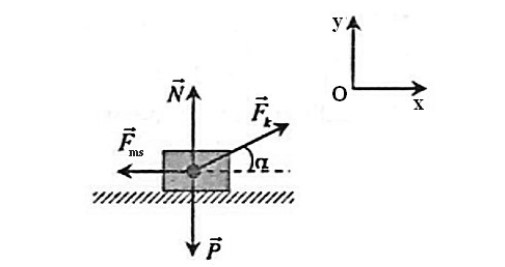
\includegraphics[scale=0.6]{../figs/VN10-2022-PH-TP021-7.jpg}
		\end{center}
		- Vật chịu tác dụng của trọng lực $P$, phản lực $N$, lực kéo $F$ và lực ma sát trượt $F_\text{ms}$. Chọn hệ trục Oxy như hình trên.
		
		- Áp dụng định luật II Newton ta có:
		
		$$\vec P + \vec N + \vec F + \vec F_\text{ms} = m\vec a.$$
		
		- Chiếu lên hệ trục ta được:
		
		$$\text{Ox}: F \cos \alpha - F_\text{ms} = ma.\ (1)$$
		
		$$\text{Oy}: - P + N + F \sin \alpha = 0 \Rightarrow N = P - F\sin \alpha.\ (2)$$
		
		$$F_\text{ms} = \mu N.\ (3)$$
		
		Từ (1), (2), (3) suy ra:
		
		$$a = \dfrac{F \cos \alpha - F_\text{ms}}{m} \approx \SI{0,58}{m/s}^2.$$
		
		Vận tốc của vật sau 5 giây
		
		$$v = at = \SI{2,9}{m/s}.$$
		
		
	} 
	\item \mkstar{3}
	
	
	{
		Hai vật $m_1 = \SI{1}{kg}$, $m_2 = \SI{0,5}{kg}$ nối với nhau bằng sợi dây và được kéo lên thẳng đứng nhờ lực $F = \SI{18}{N}$ đặt lên vật I. Tìm gia tốc chuyển động. Coi dây là không giãn và có khối lượng không đáng kể.
		\begin{center}
			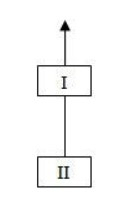
\includegraphics[scale=0.6]{../figs/VN10-2022-PH-TP021-8.jpg}
		\end{center}
	}
	
	\hideall
	{
		Các ngoại lực tác dụng lên hệ: các trọng lực $\vec P_1$, $\vec P_2$, lực kéo $\vec F$.
		
		Chọn chiều dương hướng lên. Gia tốc của hệ là:
		
		$$a = \dfrac{F - P_1 - P_2}{m_1 + m_2} = \SI{2}{m/s}^2.$$
	}
	\item \mkstar{3}
	
	
	{
		Từ chân một mặt phẳng nghiêng góc $30^\circ$ so với phương ngang, một chất điểm được truyền vận tốc đầu $\vec v_0$ hướng lên dọc theo mặt phẳng nghiêng. Hệ số ma sát giữa vật và mặt phẳng nghiêng là 0,5. Vật dừng lại ở đúng đỉnh của mặt phẳng nghiêng có độ cao $h =\SI{2}{m}.$ Lấy $ g = \SI{10}{m/s}^2$. Tìm $v_0$.
		
		\begin{center}
			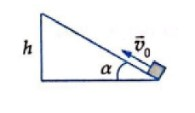
\includegraphics[scale=1]{../figs/VN10-2022-PH-TP021-9.jpg}
		\end{center}
	}
	
	\hideall
	{
		
		Các lực tác dụng lên vật như hình vẽ.
		\begin{center}
			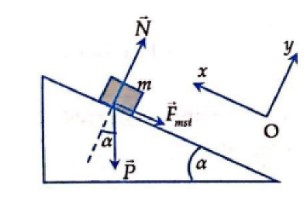
\includegraphics[scale=1]{../figs/VN10-2022-PH-TP021-10.jpg}
		\end{center}
		Áp dụng định luật II Newton:
		
		$$\vec N + \vec P + \vec F_\text{ms} = m\vec a.\ (1)$$
		
		Chọn hệ trục tọa độ Oxy như hình vẽ.
		
		Chiếu (1) lên Oy ta có:
		
		$$ - P \cos \alpha + N =0 \Rightarrow N = mg \cos \alpha\ (2).$$
		
		Chiếu (1) lên Ox ta có: 
		
		$$ - P \sin \alpha - F_\text{ms} = ma\ (3).$$
		
		Từ (2) và (3) suy ra:
		
		$$a = -g(\sin \alpha + \mu \cos \alpha).$$
		
		Quãng đường vật đi được chính bằng chiều dài mặt phẳng nghiêng:
		
		$$s = \dfrac{h}{\sin \alpha } = \SI{4}{m}.$$
		
		Áp dụng công thức:
		
		$$v^2 - v_0^2 = 2as. (v=0)$$ 
		
		Suy ra:
		
		$$v_0 = \sqrt{2g(\sin \alpha + \mu \cos \alpha)s} \approx \SI{8,6}{m/s}.$$
	}
	\item \mkstar{3}
	
	
	{
	Một ô tô có khối lượng 2 tấn đang chạy với vận tốc $v_0$ thì hãm phanh, xe đi thêm quãng đường $\SI{15}{m}$ trong $\SI{3}{s}$ thì dừng hẳn. Tính:
	\begin{enumerate}[label=\alph*)]
		\item Vận tốc $v_0$.
		\item Lực hãm phanh. Bỏ qua các lực cản bên ngoài.
	\end{enumerate}
	}
	
	\hideall
	{
		\begin{center}
			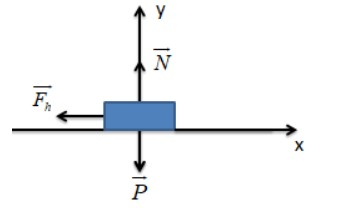
\includegraphics[scale=1]{../figs/VN10-2022-PH-TP021-11.jpg}
		\end{center}
	
		Chọn hệ trục tọa độ Oxy gắn với vật như hình vẽ.
		
		Phương trình định luật II Newton cho vật là:
		
		$$\vec P + \vec N + \vec F_\text{h} = m\vec a (*).$$
		
		Chiếu phương trình (*) lên trục Oy ta được:
		
		$$N - P = 0 \Rightarrow N = P\ (1).$$
		
		Chiếu phương trình (*) lên trục Ox ta được:
		
		$$ - F_\text{h} = ma\ (2).$$
		
		\begin{enumerate}[label=\alph*)]
			\item Áp dụng công thức của chuyển động thẳng biến đổi đều:
			
			$$\begin{cases}
				s = v_0t+ \dfrac{1}{2}at^2\ (3).\\
				v = v_0 +at\ (4).
			\end{cases}$$
		
			Thay các dữ kiện đề bài vaò (3) và (4) tìm được
			
			$$\begin{cases}
				v_0 = \SI{10}{m/s}.\\
				a = - \xsi{\dfrac{10}{3}}{m/s}^2.
			\end{cases}$$
			\item Lực hãm phanh
			
			$$F_\text{h} = -ma = \SI{6666,7}{m}.$$
		\end{enumerate}
	}
	\item \mkstar{3}
	
	
	{
		Một thiết bị vũ trụ có khối lượng $\SI{70,0}{kg}$. Khi thiết bị này cất cánh từ bề mặt Mặt Trăng, lực nâng hướng thẳng đứng, lên khỏi bề mặt Mặt Trăng do động cơ tác dụng lên thiết bị là $\SI{500}{N}$. Gia tốc rơi tự do trên bề mặt Mặt Trăng là $\SI{1,6}{m/s}^2$. Hãy xác định:
		\begin{enumerate}[label=\alph*)]
			\item  Trọng lượng của thiết bị này khi ở trên Mặt Trăng.
			
			\item Tổng hợp lực nâng của động cơ và lực hấp dẫn của Mặt Trăng tác dụng lên thiết bị.
			
			\item Gia tốc của thiết bị khi cất cánh từ bề mặt Mặt Trăng.
			
		\end{enumerate}
	}
	
	\hideall
	{
		\begin{enumerate}[label=\alph*)]
			\item  Trọng lượng của thiết bị này khi ở trên Mặt Trăng
			
			$$P = mg = \SI{112}{N}.$$
			
			\item Ta có:
			
			- Lực nâng của động cơ: $F_\text{n} = \SI{500}{N}.$
			
			- Lực hấp dẫn của Mặt Trăng tác dụng lên thiết bị: $P = \SI{112}{N}.$
			
			Hai lực này cùng phương, ngược chiều.
			
			- Tổng hợp lực nâng của động cơ và lực hấp dẫn của Mặt Trăng tác dụng lên thiết bị là:
			
			$$F = F_\text{n} - P = \SI{388}{N}.$$
			
			\item Gia tốc của thiết bị khi cất cánh từ bề mặt Mặt Trăng
			
			$$a = \dfrac{F}{m} = \SI{5,53}{m/s}^2.$$
			
		\end{enumerate}
	}
	\item \mkstar{3}
	
	
	{
		Hai vật giống nhau, mỗi vật có trọng lượng $P$, đặt chồng lên nhau. Vật trên được buộc vào tường bằng một sợi dây. Vật dưới được kéo sang phải bằng một lực $F$ nằm ngang (H.II.1).Hệ số ma sát trượt giữa các mặt tiếp xúc là $\mu_\text{t}$. Hỏi lực $F$ phải lớn hơn giá trị nào dưới đây thì vật dưới bắt đầu trượt? Cho rằng lực ma sát nghỉ cực đại bằng lực ma sát trượt.
		
		\begin{center}
			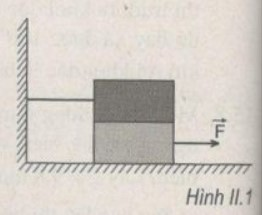
\includegraphics[scale=0.8]{../figs/VN10-2022-PH-TP021-15.jpg}
		\end{center}
	
	}
	
	\hideall
	{
		\begin{center}
			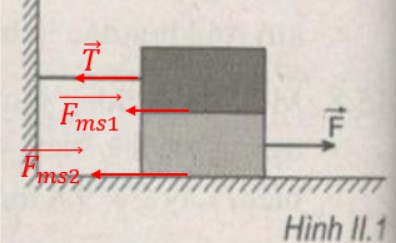
\includegraphics[scale=0.6]{../figs/VN10-2022-PH-TP021-16.jpg}
		\end{center}
	
		Vật chịu hai lực ma sát ở hai mặt tiếp xúc trên và dưới (hình vẽ).
		
		Ta có:
		
		$$\begin{cases}
			F_\text{ms1} = \mu_\text{t}N_1 =  \mu_\text{t}P_1 = \mu_\text{t}P.\\
			F_\text{ms2} = \mu_\text{t}N_2 =  \mu_\text{t}(P_1 + P_2) = 2\mu_\text{t}P.
		\end{cases} \Rightarrow F_\text{ms1} + F_\text{ms2} = 3\mu_\text{t} P.$$
	
	Vậy để vật dưới bắt đầu trượt thì
	
	$$F > F_\text{ms1} + F_\text{ms2} \Rightarrow F > 3\mu_\text{t} P.$$
		
	
	}
	
	\item \mkstar{3}
	
	
	{
		Một cái hòm khối lượng $m = \SI{40}{kg}$ đặt trên sàn nhà. Hệ số ma sát trượt giữa hòm và sàn nhà là $\mu_\text{t} = \SI{0,2}{}$. Người ta đẩy hòm bằng một lực $F =200N$ theo phương hợp với phương nằm ngang một góc $\alpha = 30^\circ$, chếch xuống phía dưới. Tính gia tốc của hòm. 
		
		\begin{center}
			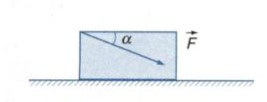
\includegraphics[scale=1]{../figs/VN10-2022-PH-TP021-17.jpg}
		\end{center}
	}
	
	\hideall
	{
		Vật chịu tác dụng của 4 lực được biểu diễn như hình vẽ.
		
		\begin{center}
			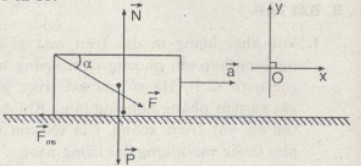
\includegraphics[scale=1]{../figs/VN10-2022-PH-TP021-18.jpg}
		\end{center}
	
		Áp dụng định luật II Newton ta có :
		
			$$\vec F + \vec F_\text{ms} + \vec P + \vec N = m\vec a.$$
		
		Chiếu lên hệ trục tọa độ:
		
		$$\begin{cases}
			\text{Ox:}  F\cos \alpha - F_\text{ms} =ma.\ (1) \\
			\text{Oy:}   - P + N - F\sin \alpha= 0 \Rightarrow N =mg + F \sin \alpha\ (2).
			
		\end{cases}$$
		
		Thay (2) vào (1) ta được:
		
		$$ a = \dfrac{F \cos \alpha - \mu (mg + F\sin \alpha)}{m} = \SI{1,87}{m/s}^2. $$
	
	}
	\item \mkstar{3}
	
	
	{
		Một vật đặt trên mặt phẳng nghiêng (góc nghiêng $\alpha = 30^\circ$), được truyền một vận tốc ban đầu $v_0 = \SI{2}{m/s}$. Hệ số ma sát giữa vật và mặt phẳng nghiêng là 0,3. Tính gia tốc của vật.
		\begin{center}
			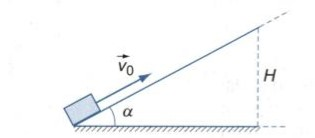
\includegraphics[scale=1]{../figs/VN10-2022-PH-TP021-20.jpg}
		\end{center}
	}
	
	\hideall
	{
		\begin{center}
			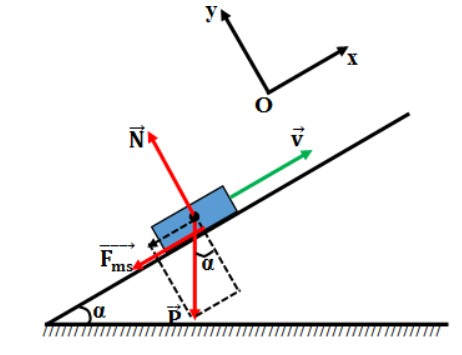
\includegraphics[scale=0.6]{../figs/VN10-2022-PH-TP021-21.jpg}
		\end{center}
	
		Áp dụng định luật II Newton ta có: 
		
		$$\vec P + \vec N + \vec F_\text{ms} = m\vec a (*).$$
		
		Chiếu (*) lên Ox: 
		
		$$-P_\text{x} – F_\text{ms} = ma \Rightarrow - mg\sin \alpha - \mu N = ma\ (1).$$
		
		Chiếu (*) lên Oy: 
		
		$$-P_\text{y} + N = 0 \Rightarrow N = P_\text{y} = P\cos \alpha.\ (2)$$
		
		Thay (2) vào (1) suy ra:
		
		$$a = -g (\sin \alpha +  \mu \cos \alpha) = - \SI{7,45}{m/s}^2.$$
		
	}

	

	\item \mkstar{3}
	
	
	{
		Người ta vắt qua một chiếc ròng rọc nhẹ một đoạn dây, ở hai đầu có treo hai vật A và B có khối lượng là $m_\text{A} =\SI{260}{g}$ và $m_\text{B} = \SI{240}{g}$ . Thả cho hệ bắt đầu chuyển động. Tính gia tốc của hệ vật.
		
		\begin{center}
			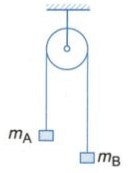
\includegraphics[scale=1]{../figs/VN10-2022-PH-TP021-22.jpg}
		\end{center}
		}

	\hideall{
	\begin{center}
	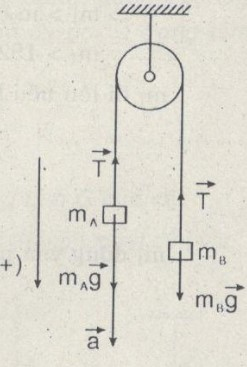
\includegraphics[scale=0.6]{../figs/VN10-2022-PH-TP021-23.jpg}
	\end{center}

		Chọn chiều dương là chiều chuyển động của hai vật.
		
		Áp dụng định luật II Newton:
		
		$$\vec P_1 + \vec T_1 = m_1 \vec a \Rightarrow P_1 - T_1 = m_1a\ (1).$$
		
		$$\vec P_2 + \vec T_2 = m_2 \vec a \Rightarrow - P_2 - T_2 = m_2a\ (2).$$
		
		Lấy (1) cộng (2) vế theo vế
		
		$$ P_1 - P_2 = m_1 a + m_2 a = (m_1+ m_2)a \Rightarrow a = \dfrac{P_1 - P_2}{m_1 + m_2} = \SI{0,4}{m/s}^2.$$
		
	}
	\item \mkstar{3}
	
	
	{
		Một ô tô đang chuyển động với vận tốc $\SI{10}{m/s}$ thì tắt máy, chuyển động chận dần đều do ma sát, hệ số ma sát giữa bánh xe và mặt đường là 0,5. Tính gia tốc, thời gian và quãng đường chuyển động chậm dần đều?
	}
	
	\hideall
	{
		Chọn chiều dương là chiều chuyển động.
		
		Áp dụng định luật II Newton cho vật trượt theo phương ngang:
		
		$$- F_\text{ms} = ma \Rightarrow - \mu mg = ma \Rightarrow a = - mu g = - \SI{5}{m/s}^2.$$
		
		Thời gian và quãng đường chuyển động chậm dần
		
		$$s = \dfrac{-v_0^2}{2a} = \SI{10}{m}.$$
		
		$$ t = - \dfrac{v_0}{a} =\SI{2}{s}.$$ 
	}
	\item \mkstar{3}
	
	
	{
		Một ô tô có khối lượng 1 tấn, chuyển động trên đường nằm ngang. Hệ số ma sát lăn giữa bánh xe và mặt đường là 0,1. Tính lực kéo của động cơ nếu
		
		\begin{enumerate}[label=\alph*)]
			\item Ô tô chuyển động thẳng đều.
			\item Ô tô chuyển động nhanh dần đều với gia tốc $\SI{2}{m/s}^2$.
		\end{enumerate}
	}
	
	\hideall
	{
		Chọn chiều dương là chiều chuyển động.
		
		Áp dụng định luật II Newton cho vật trượt theo phương ngang:
		
		$$F - F_\text{ms} = ma \Rightarrow F = ma + F_\text{ms} = ma + \mu mg.$$
		\begin{enumerate}[label=\alph*)]
			\item  Lực kéo của động cơ nếu ô tô chuyển động thẳng đều ($a=0$)
			
			$$F = F_\text{ms} = \SI{1000}{N}.$$ 
			
			\item Lực kéo của động cơ nếu ô tô chuyển động nhanh dần đều với gia tốc $\SI{2}{m/s}^2$
			
			$$F = ma + F_\text{ms} = ma + \mu mg = \SI{3000}{N}.$$
		\end{enumerate}
	}
	\item \mkstar{3}
	
	
	{
		Một đầu máy tạo ra lực kéo để kéo một toa xe có khối lượng 4 tấn chuyển động với gia tốc $a = \SI{0,4}{m/s}^2$. Biết hệ số ma sát giữa toa xe và mặt đường là $\mu = \text{0,02}$. Hãy xác định lực kéo của đầu máy? Lấy $g = \SI{10}{m/s}^2$.
	}
	
	\hideall
	{
		Chọn chiều dương là chiều chuyển động.
		
		Áp dụng định luật II Newton cho vật trượt theo phương ngang:
		
		$$F - F_\text{ms} = ma \Rightarrow F = ma + F_\text{ms} = ma + \mu mg = \SI{2400}{N}.$$
	}
		\item \mkstar{4}
	
	
	{Cho cơ hệ như hình vẽ.
		\begin{center}
			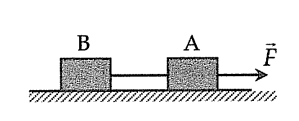
\includegraphics[scale=0.8]{../figs/VN10-2021-PH-TP012-1.png}
		\end{center}
		Vật A có khối lượng $m_1=200\ \text g$, vật B có khối lượng $m_2=120\ \text g$ nối với nhau bởi một sợi dây nhẹ, không dãn. Hệ số ma sát trượt giữa hai vật và mặt phẳng ngang là $\mu = 0,4$. Tác dụng vào A một lực kéo $\vec F$ theo phương ngang. Biết rằng dây nối hai vật chỉ chịu được lực căng tối đa $T_0=0,6\ \text N$. Lấy $g=10\ \text{m/s}^2$. Tìm lực $F$ lớn nhất để dây không bị đứt.
	}
	
	\hideall
	{	\begin{center}
			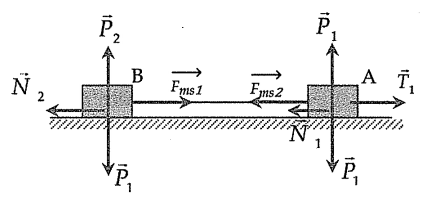
\includegraphics[scale=0.8]{../figs/VN10-2021-PH-TP012-2.png}
		\end{center}
		
		Áp dụng định luật II Niu-tơn cho hệ vật:
		\[F-\mu (m_1 + m_2)g=(m_1+m_2)a \Rightarrow a = \dfrac{F}{m_1 + m_2} - \mu g\]
		
		Áp dụng định luật II Niu-tơn cho vật B:
		\[T-\mu m_2g=m_2 a \Rightarrow T = (\mu g + a)m_2 = \dfrac{F m_2}{m_1 + m_2} \Rightarrow F = \dfrac{m_1 + m_2}{m_2}T\]
		
		Do dây chỉ chịu được lực căng tối đa $0,6\ \text N$, nên thay số ta tính được $F$ tối đa là $F=1,6\ \text N$.
	}
	\item \mkstar{4}
	
	
	{Cho cơ hệ như hình vẽ.
		\begin{center}
			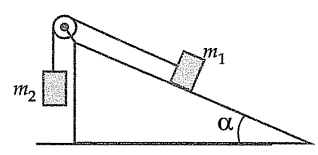
\includegraphics[scale=0.8]{../figs/VN10-2021-PH-TP012-3.png}
		\end{center}
		Mặt phẳng nghiêng cố định, nghiêng góc $\alpha$ so với phương ngang. Hai chất điểm khối lượng $m_1$, $m_2$ được nối với nhau bởi dây nhẹ, không dãn vắt qua ròng rọc nhẹ có kích thước không đáng kể. Biết rằng $m_2 > m_1 \sin \alpha$. Bỏ qua mọi ma sát, cho gia tốc trọng trường là $g$. Thả hai vật chuyển động tự do, tìm gia tốc của mỗi vật.
	}
	
	\hideall
	{	\begin{center}
			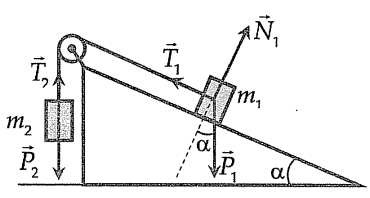
\includegraphics[scale=0.8]{../figs/VN10-2021-PH-TP012-4.png}
		\end{center}
		
		Do $m_2 > m_1 \sin \alpha$ nên $m_2$ sẽ đi xuống.
		
		Áp dụng định luật II Niu-tơn cho mỗi vật:
		\begin{align*}
			\vec T_1 + \vec N + \vec P_1 &= m_1 \vec a_1 \\
			\vec T_2 + \vec P_2 &= m_2 \vec a_2
		\end{align*}
		
		Do dây nhẹ, không dãn, ròng rọc không khối lượng nên $T_1 = T_2 = T$, $a_1 = a_2 = a$.
		
		Chiếu các vectơ lên phương chuyển động của mỗi vật, ta được:
		\begin{align*}
			T - P_1 \sin \alpha &= m_1 a \\
			-T + P_2 &= m_2 a
		\end{align*}
		
		Suy ra $a=\dfrac{m_2 - m_1 \sin \alpha}{m_1 + m_2}g$.
	}
\end{enumerate}